\section{Data life cycle}

\begin{frame}{Data life cycle scheme}
\centering
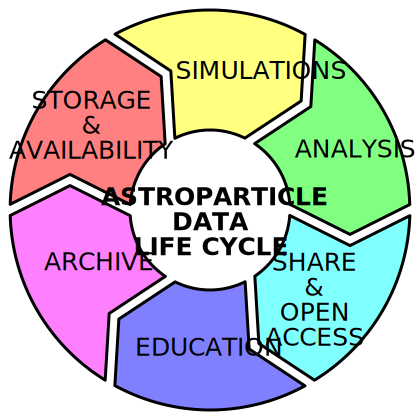
\includegraphics[width=0.6\textwidth]{pics/ADLC.pdf}
\end{frame}

\subsection{Archiving and storage}

\begin{frame}{Data-oriented approach}
% \vspace{-1em}
What data do we work with?

% \vspace{3em}

\parbox{0.48\textwidth}{
\begin{itemize}
  \item Data types:
  \begin{itemize}
    \item Raw detector readouts;
    \item Pre-analyzed events;
    \item Metadata
  \end{itemize}
\end{itemize}
}
\hfill
\parbox{0.48\textwidth}{
\begin{itemize}
  \item Data structure:
  \begin{itemize}
    \item Different formats;
    \item Different messengers;
    \item Common metadata
  \end{itemize}
\end{itemize}
}

Our approach:
\begin{itemize}
 \item It is proposed to store unique event id and metadata in the unified database
 \item With growing data sizes, distribured storage for events\\could be useful
\end{itemize}
\insimg{ADLC0.pdf}
\end{frame}

\begin{frame}{Archiving and storage}
\centering
\includegraphics[width=0.62\textwidth]{pics/data_workflow_4.pdf}
% \begin{itemize}
% \item Bad way / good way;
% \item Distributed storage as a solution on top of existing servers (see Nguen);
% \item Acquisition by metadata;
% \item What is metadata?
% \end{itemize}
\insimg{ADLC0.pdf}
\end{frame}

\begin{frame}{Proposed cosmic-ray metadata structure}
\vspace{-1.5em}
\begin{center}
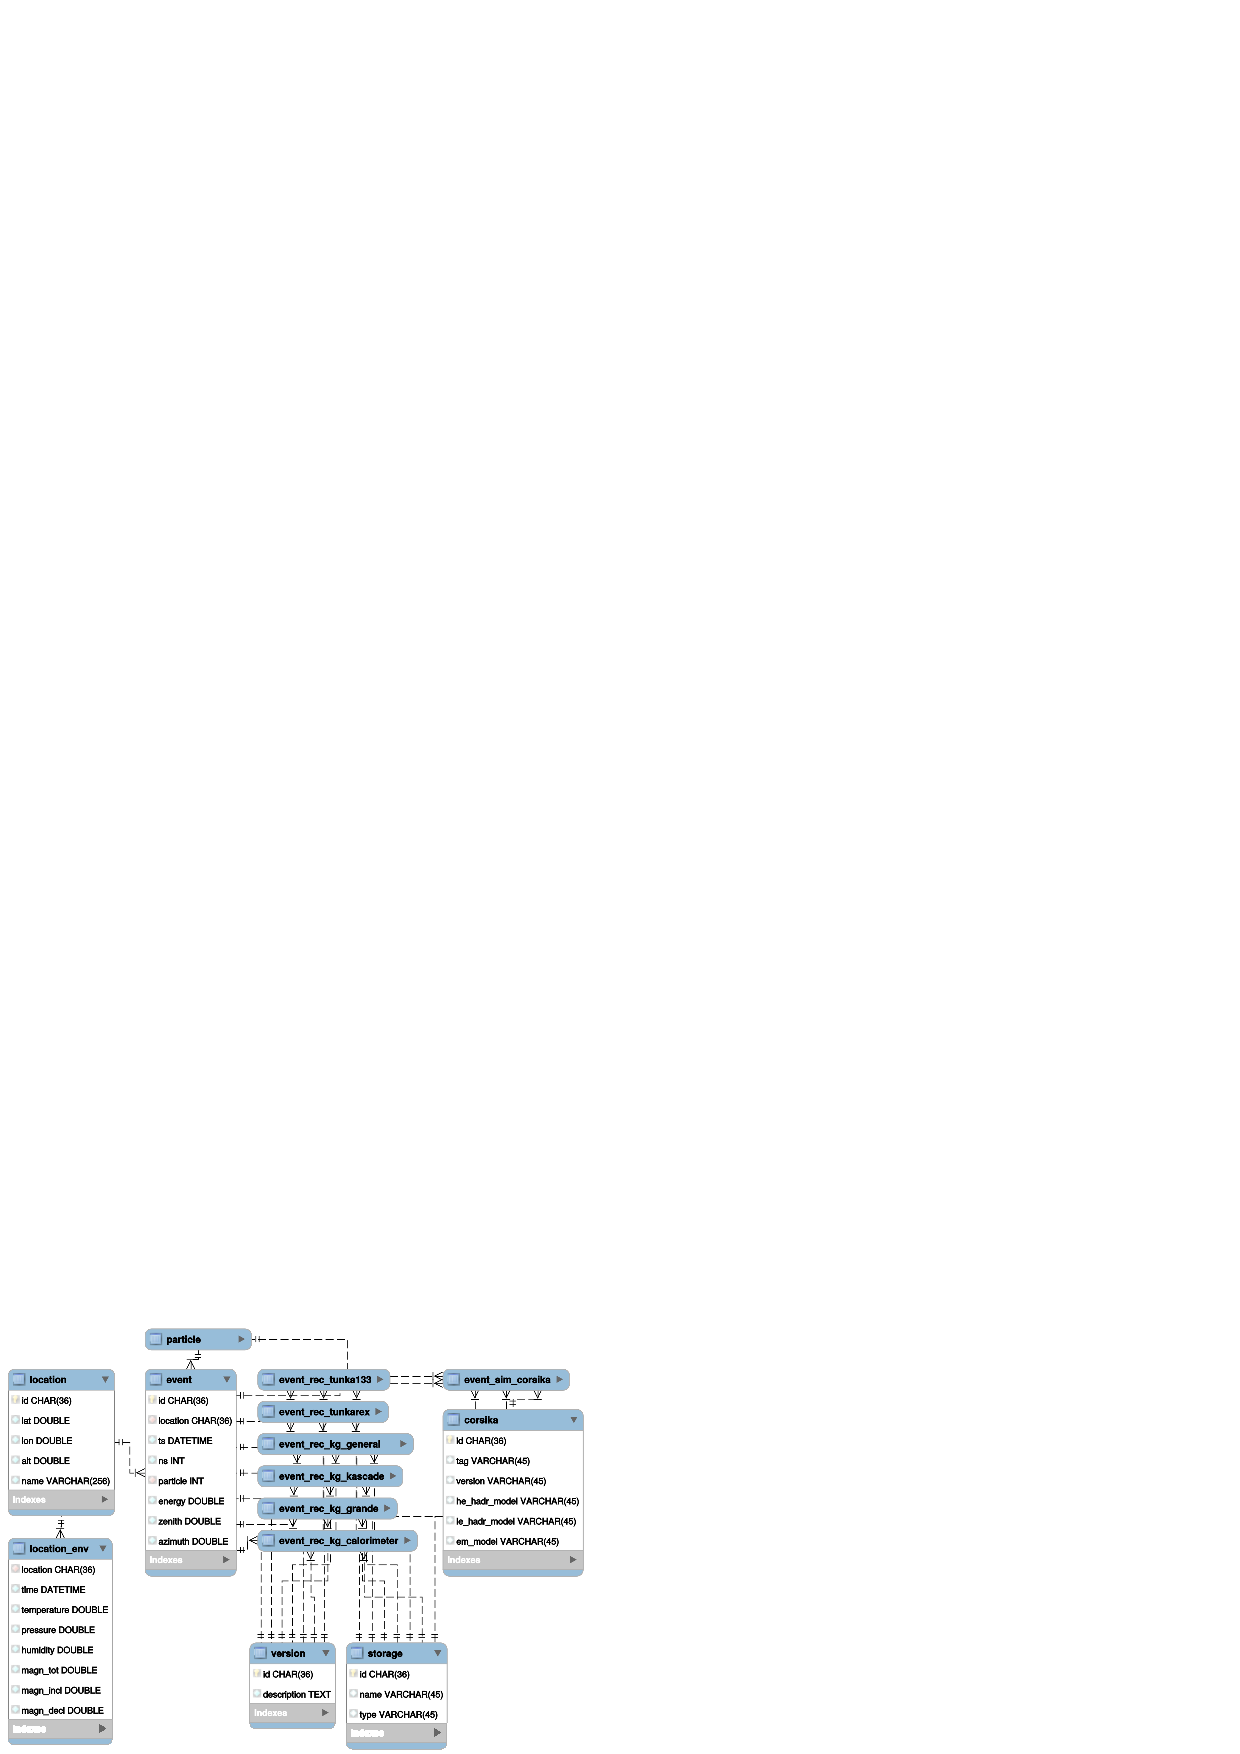
\includegraphics[width=0.82\textwidth]{pics/metadata.pdf}
\end{center}
\insimg{ADLC0.pdf}
\end{frame}

\subsection{Simulation and analysis}

\begin{frame}{Data workflow}
\vspace{-2em}
\centering
\only<1>{\includegraphics[width=1\textwidth]{pics/KRAD_workflow_curr.pdf}}
\only<2>{\includegraphics[width=1\textwidth]{pics/KRAD_workflow_hori.pdf}}
\insimg{ADLC1.pdf}
\end{frame}

\begin{frame}{Simulation}
\begin{block}{Simulation: two steps}
\begin{enumerate}
\item Simulating EAS:
  \begin{itemize}
  \item CORSIKA, does not depend on detector features, depends on location ans atmospheric conditions;
  \item requires large computing power with a standard environment;
  \item a small amount of input data and a large amount of output data;
  \end{itemize}
\item Simulating detector output:
  \begin{itemize}
  \item depends on detector features;
  \item requires dedicated software and special environment for it;
  \item large amount of both input and output data;
  \end{itemize}
\end{enumerate}
\end{block}
\insimg{ADLC1.pdf}
\end{frame}

\begin{frame}{Analysis}
% \begin{block}{Steps}
% \begin{itemize}
% \item Event building;
% \item Data calibration and correction;
% \item Preliminary reconstruction of shower variables;
% \item Data mapping and scaling;
% \item Final reconstruction;
% \item Joint data analysis.
% \end{itemize}
% \end{block}
\includegraphics[width=1\textwidth]{pics/an_steps.pdf}
\vspace{2em}

\begin{itemize}
\item Analysis could be either algorithmic or machine learning;
\item Machine learning requires large enough statistics\\in order to work properly.
\end{itemize}
\insimg{ADLC1.pdf}
\end{frame}

\begin{frame}{Analysis features}
\vspace{-3em}
\begin{block}{Software for data analysis depends on a particular experiment}
  \begin{itemize}
    \item Problem: It may even require dedicated system environment
    \item \textbf{Solution: Virtualization\footnotemark[2]}
  \end{itemize}
\end{block}

\begin{block}{Data analysis requires huge amounts of input data}
  \begin{itemize}
    \item Problem: It is often more optimal to perform it on the same site the data are stored
    \item \textbf{Solution: Job management}
  \end{itemize}
\end{block}
\insimg{ADLC1.pdf}
  \footnotesize\footnotetext[2]{``The act of creating a virtual (rather than actual) 
  version of something,\\ \hspace{1.5em}including virtual computer hardware platforms, 
  storage devices,\\ \hspace{1.5em}and computer network resources''. $\copyright$ Wikipedia}
\end{frame}

\begin{frame}{WMS---workload management system}
\begin{itemize}
  \item The basic idea is to provide a central queue for all users and make all the distributed sites look like local ones;
  \item Starting from mid 90's are widely used in collider experiments (Dirac, PanDA);
  \item Dedicated for:
  \begin{itemize}
  \item Unified usage of the distributed remote data and common data analysis;
  \item Conceal various low-level software and provide unified high-level interface;
  \end{itemize}
%   \item
%   Hide middleware while supporting diversity and evolution
%   \begin{itemize}
%     \item WMS interacts with middleware, users see only high level workflow
%     \item Automation engines built in WMS, not exposed to users
%   \end{itemize}
  \item Provide the common way to issue tasks to different\\types of the distibuted sites;
  \item
%   Use the same system for simulation, data processing and users analysis
  The same system for the data access, analysis and\\simulation.
%   \item Similar ideas have been implemented in several independent systems developed by LHC experiments: AliEn, Dirac, PanDA
\end{itemize}
\insimg{ADLC1.pdf}
\end{frame}

\begin{frame}{WMS for astroparticle data management}
\begin{itemize}
 \item <2->IceCube ? \onslide<3->{PanDa}
 \item <4-> Auger ? \onslide<5->{DiRAC}
 \item <6-> Other WMS ? \onslide<7->{VCondor, MyCluster, GWPilot, BigJob, ...}
 \vspace{2em}
 \item <8-> \textbf{\textcolor{kit-green100}{APPDC - ?}}
\end{itemize}

% \begin{center}
% \fbox{
%   \parbox[c][0.4\textheight]{0.8\textwidth}{
%     \Huge\centering
%     Here be a cloud\\of various WMS's.
%   }
% }
% \end{center}


% My task is to develop and deploy distributed execution\\for simulation and analysis jobs.
\insimg{ADLC1.pdf}
\end{frame}

\subsection{Open access and education}

\begin{frame}{Open access and education}
\vspace{-4em}
\begin{itemize}
\item Open access: a dedicated portal planned;
\item Education: \textcolor{blue}{\texttt{astroparticle.online}}.
\end{itemize}
\centering
\includegraphics[width=0.85\textwidth]{pics/astro_onl.png}
\insimg{ADLC2.pdf}
\end{frame}
